\chapter{Preámbulo}
    \section{¿Quiénes somos?}
        \begin{table}[!ht]
            \begin{tblr}{c c}
                \SetCell[r=10]{} 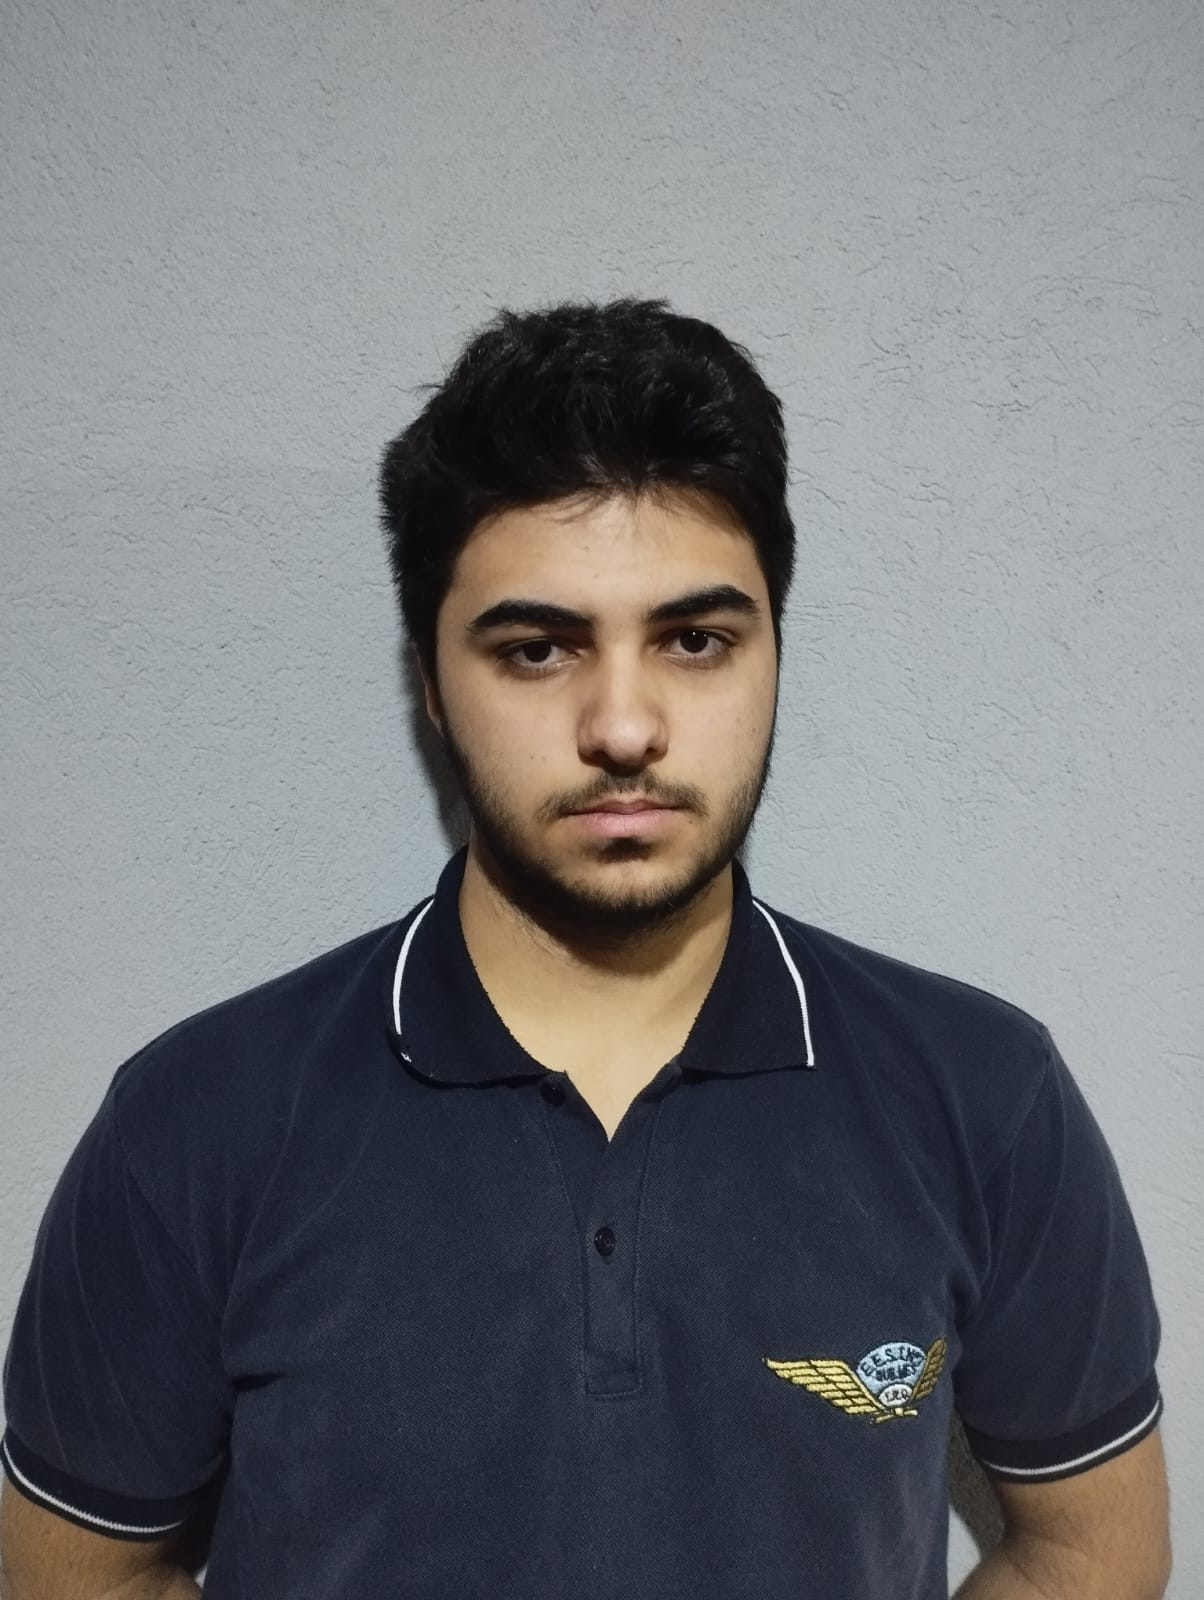
\includegraphics[width=0.25\textwidth]{Preámbulo/Fausto.png} 
                & \SetCell[r=1]{l} Fausto Alvarez Mollo
                &  \\ 
                &  \\
                & \SetCell[r=1]{l}DNI: 46635570
                & \\ 
                &  \\
                & \SetCell[r=1]{l}Mail: faustoalvarezmollo@gmail.com
                &  \\
                &  \\
                & \SetCell[r=1]{l}
\includegraphics[width=0.5cm]{Preámbulo/Linkedin.png}\href{https://www.linkedin.com/in/fausto-alvarez-mollo/}{Linkedin}
                &  \\
                &  \\
                    & \SetCell[r=1]{l}Desarrollo de electrónica y documentación.
                &  \\ 
                &  \\
            \end{tblr}
        \end{table}
        \begin{table}[!ht]
            \begin{tblr}{c c}
                \SetCell[r=10]{} 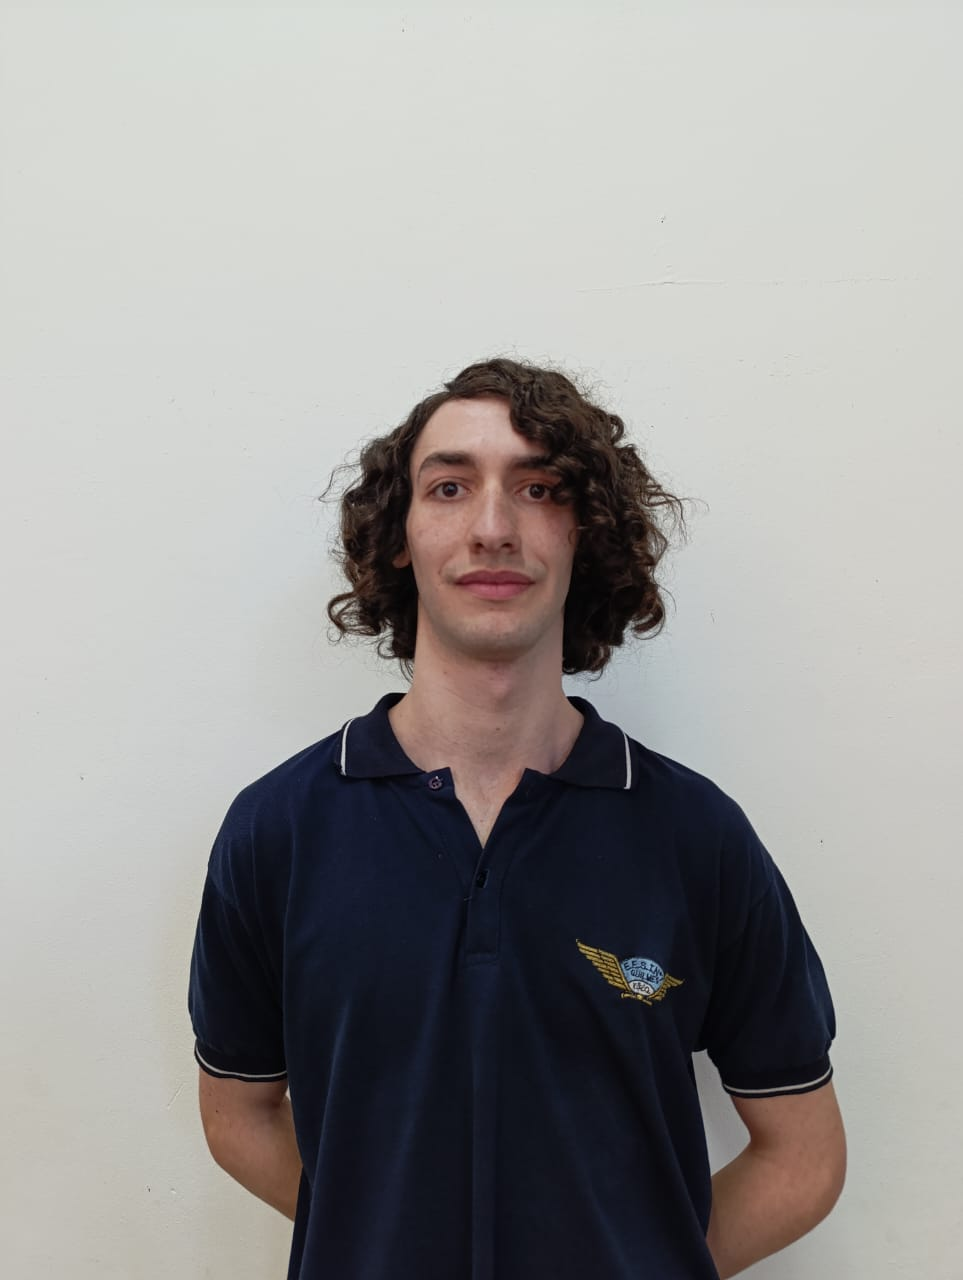
\includegraphics[width=0.25\textwidth]{Preámbulo/Mariano.png} 
                & \SetCell[r=1]{l} Mariano Joaquín Bianqui Kronemberger
                &  \\ 
                &  \\
                & \SetCell[r=1]{l}DNI: 47337141
                & \\ 
                &  \\
                & \SetCell[r=1]{l}Mail: marianobianqui@gmail.com  
                &  \\
                &  \\
                & \SetCell[r=1]{l}
\includegraphics[width=0.5cm]{Preámbulo/Linkedin.png}\href{https://www.linkedin.com/in/mariano-bianqui-5035bb303//}{Linkedin}  
                &  \\
                &  \\
                    & \SetCell[r=1]{l}Desarrollo de Página Web.
                &  \\ 
                &  \\
            \end{tblr}
        \end{table}
        \begin{table}[!ht]
                \begin{tblr}{c c}
                    \SetCell[r=10]{} 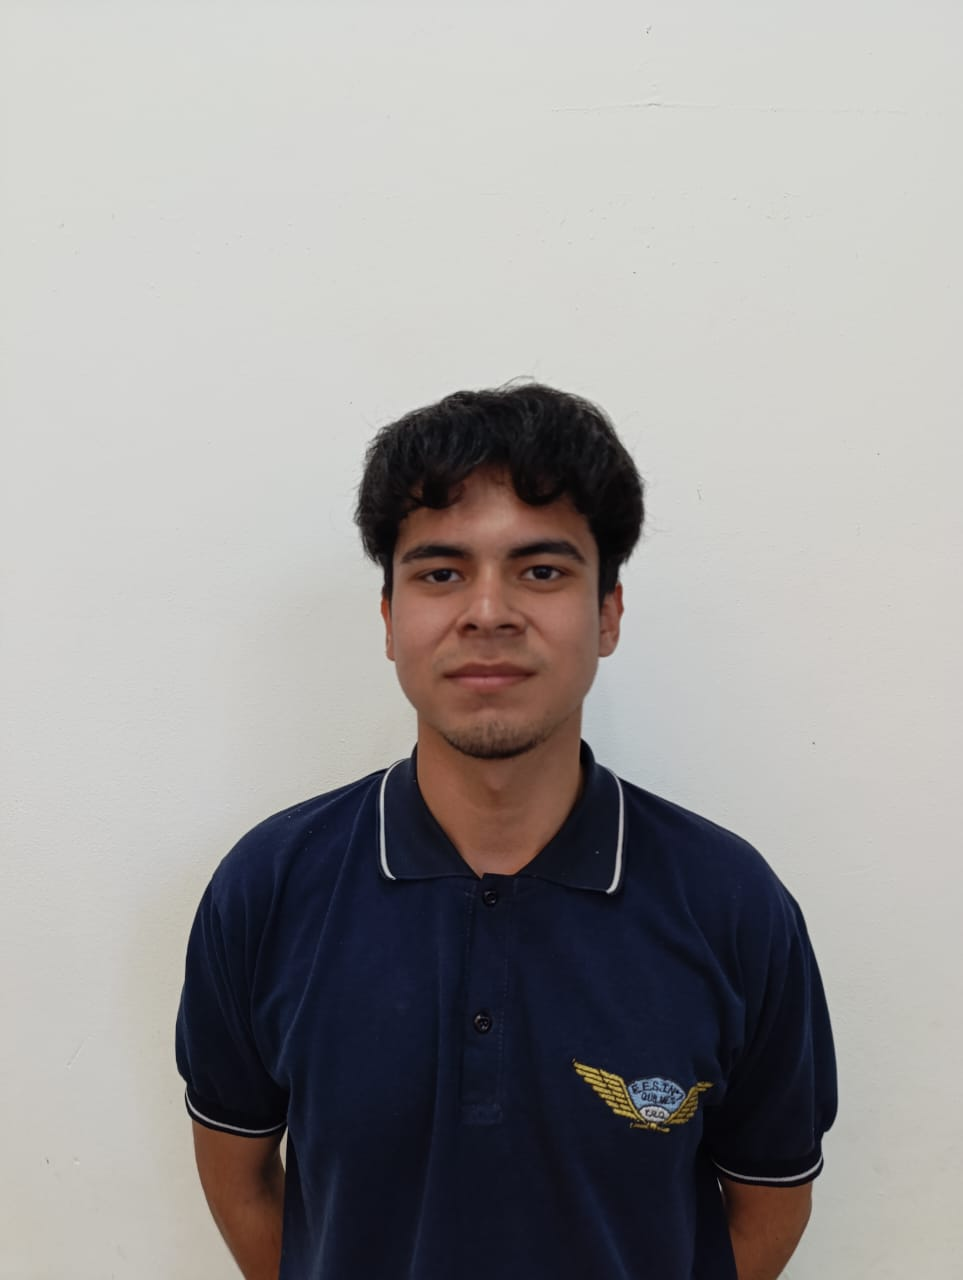
\includegraphics[width=0.25\textwidth]{Preámbulo/Tomás.png} 
                    & \SetCell[r=1]{l} Tomás Joaquín Calleja
                    &  \\ 
                    &  \\
                    & \SetCell[r=1]{l}DNI: 47031210
                    & \\ 
                    &  \\
                    & \SetCell[r=1]{l}Mail: tomascalleja918@gmail.com  
                    &  \\
                    &  \\
                    & \SetCell[r=1]{l}
\includegraphics[width=0.5cm]{Preámbulo/Linkedin.png}\href{https://www.linkedin.com/in/tomás-calleja-5a9894302/}{Linkedin}  
                    &  \\
                    &  \\
                    & \SetCell[r=1]{l}Desarrollo de Aplicación Móvil.
                    &  \\ 
                    &  \\
                \end{tblr}
            \end{table}
            \newpage
            \begin{table}[!ht]
                \begin{tblr}{c c}
                    \SetCell[r=10]{} 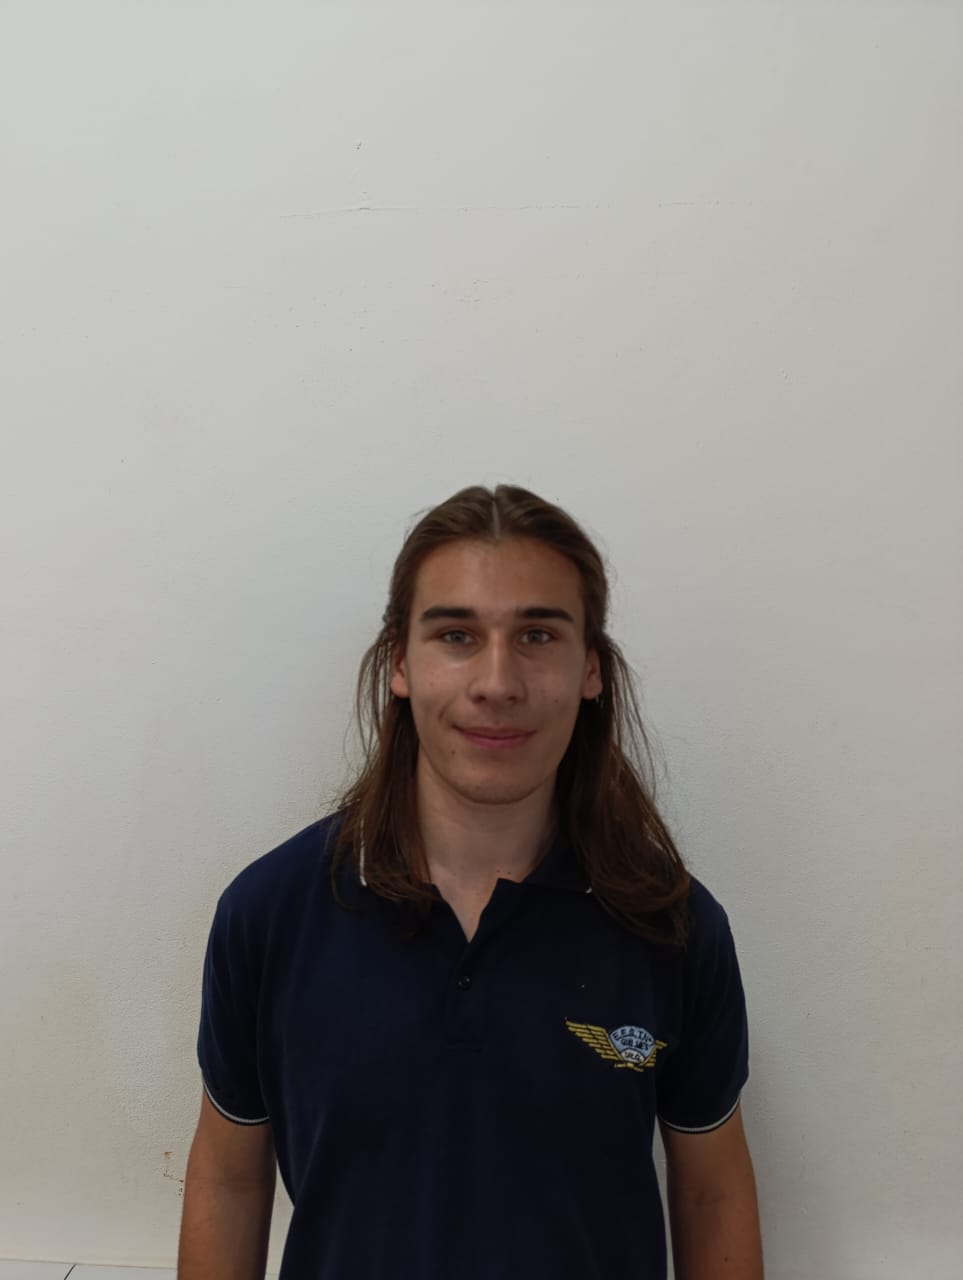
\includegraphics[width=0.25\textwidth]{Preámbulo/Augusto.png} 
                    & \SetCell[r=1]{l} Augusto Donatti
                    &  \\ 
                    &  \\
                    & \SetCell[r=1]{l}DNI: 47057413
                    & \\ 
                    &  \\
                    & \SetCell[r=1]{l}Mail: adonatti2005@gmail.com  
                    &  \\
                    &  \\
                    & \SetCell[r=1]{l}
\includegraphics[width=0.5cm]{Preámbulo/Linkedin.png}\href{https://www.linkedin.com/in/augusto-donatti-54a5bb303/}{Linkedin}
                    &  \\
                    &  \\
                        & \SetCell[r=1]{l}Desarrollo de la Estructura.
                    &  \\ 
                    &  \\
                \end{tblr}
            \end{table}
            \begin{table}[!ht]
                \begin{tblr}{c c}
                    \SetCell[r=10]{} 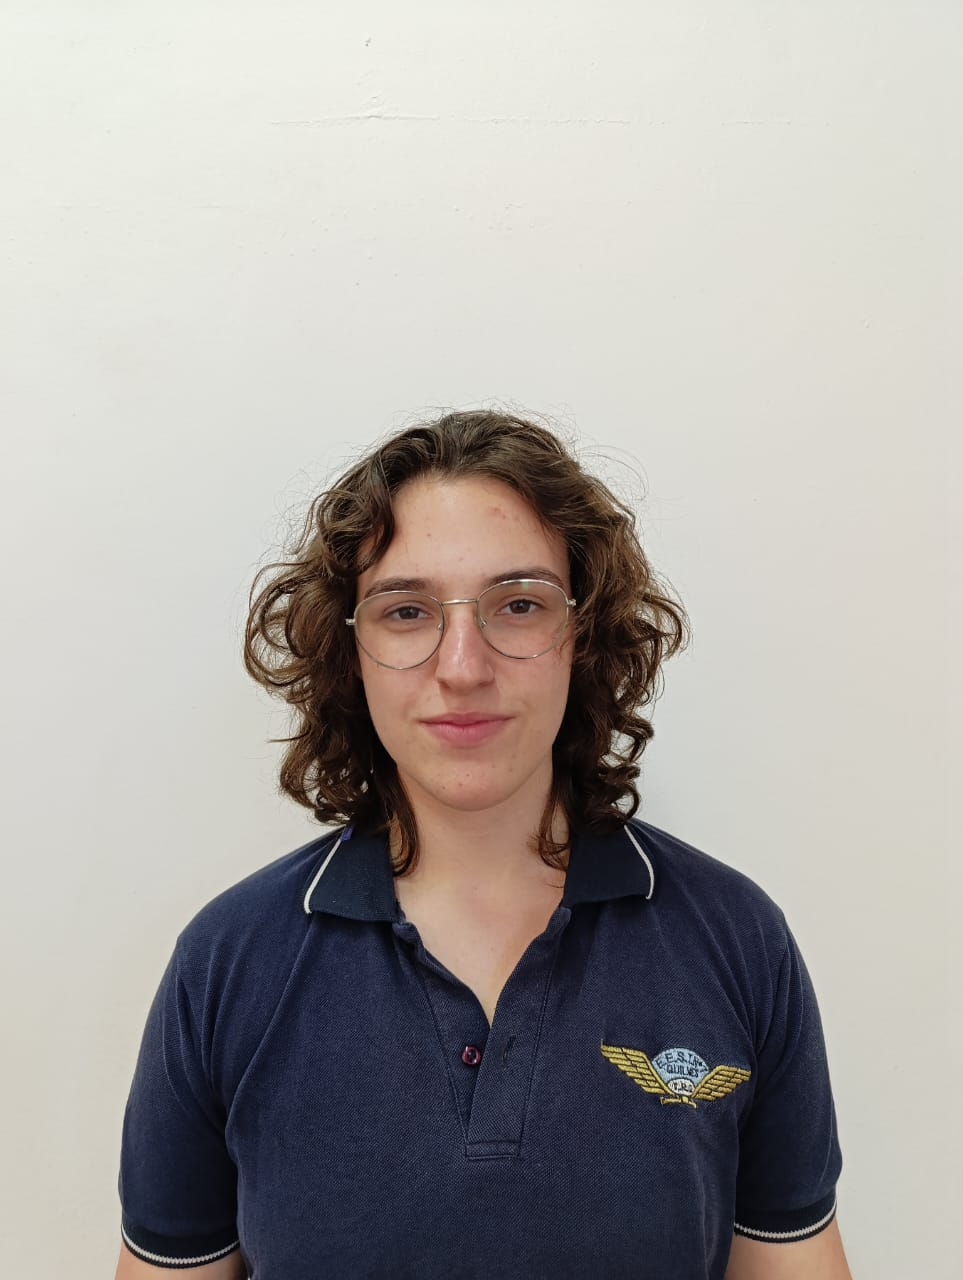
\includegraphics[width=0.25\textwidth]{Preámbulo/Tatiana.png} 
                    & \SetCell[r=1]{l} Tatiana Milena Felizia
                    &  \\ 
                    &  \\
                    & \SetCell[r=1]{l}DNI: 47144482
                    & \\ 
                    &  \\
                    & \SetCell[r=1]{l}Mail: tatianafelizia@gmail.com  
                    &  \\
                    &  \\
                    & \SetCell[r=1]{l}
\includegraphics[width=0.5cm]{Preámbulo/Linkedin.png}\href{https://www.linkedin.com/in/tatiana-felizia-9b29141bb/}{Linkedin}  
                    &  \\
                    &  \\
                        & \SetCell[r=1]{l}Desarrollo de Software e Interfaz.
                    &  \\ 
                    &  \\
                \end{tblr}
            \end{table}
            \begin{table}[!ht]
                \begin{tblr}{c c}
                    \SetCell[r=10]{} 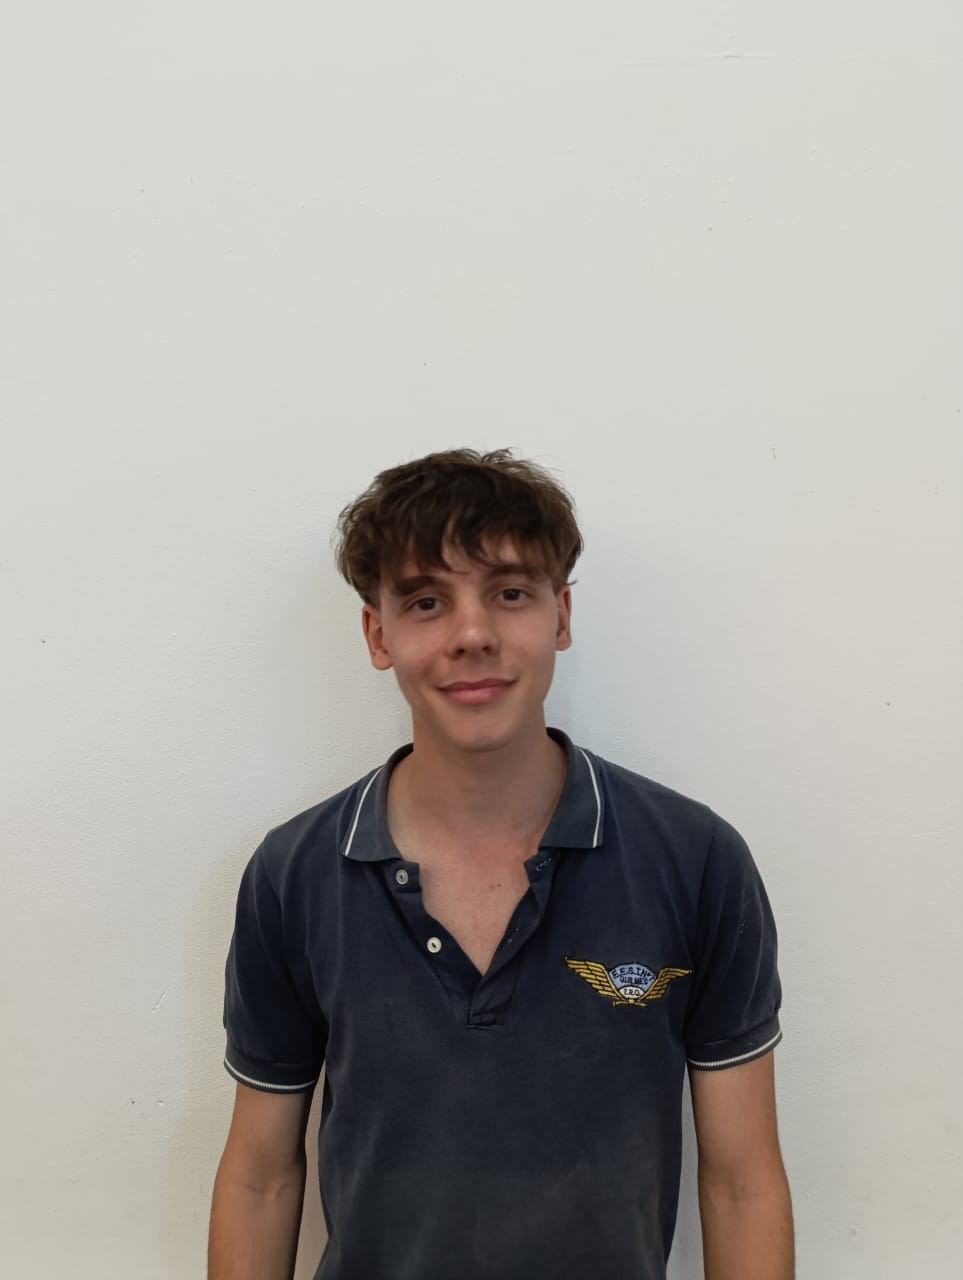
\includegraphics[width=0.25\textwidth]{Preámbulo/Gabriel.png} 
                    & \SetCell[r=1]{l} Gabriel Jerónimo Takashi Sofía
                    &  \\ 
                    &  \\
                    & \SetCell[r=1]{l}DNI: 46904826
                    & \\ 
                    &  \\
                    & \SetCell[r=1]{l}Mail: gabrielsofia19@gmail.com  
                    &  \\
                    &  \\
                    & \SetCell[r=1]{l}
\includegraphics[width=0.5cm]{Preámbulo/Linkedin.png}\href{https://www.linkedin.com/in/gabriel-sofia-035335299/}{Linkedin}  
                    &  \\
                    &  \\
                        & \SetCell[r=1]{l} Desarrollo de Marketing.
                    &  \\ 
                    &  \\
                \end{tblr}
            \end{table}
            
            \begin{figure} [H]
                \centering
                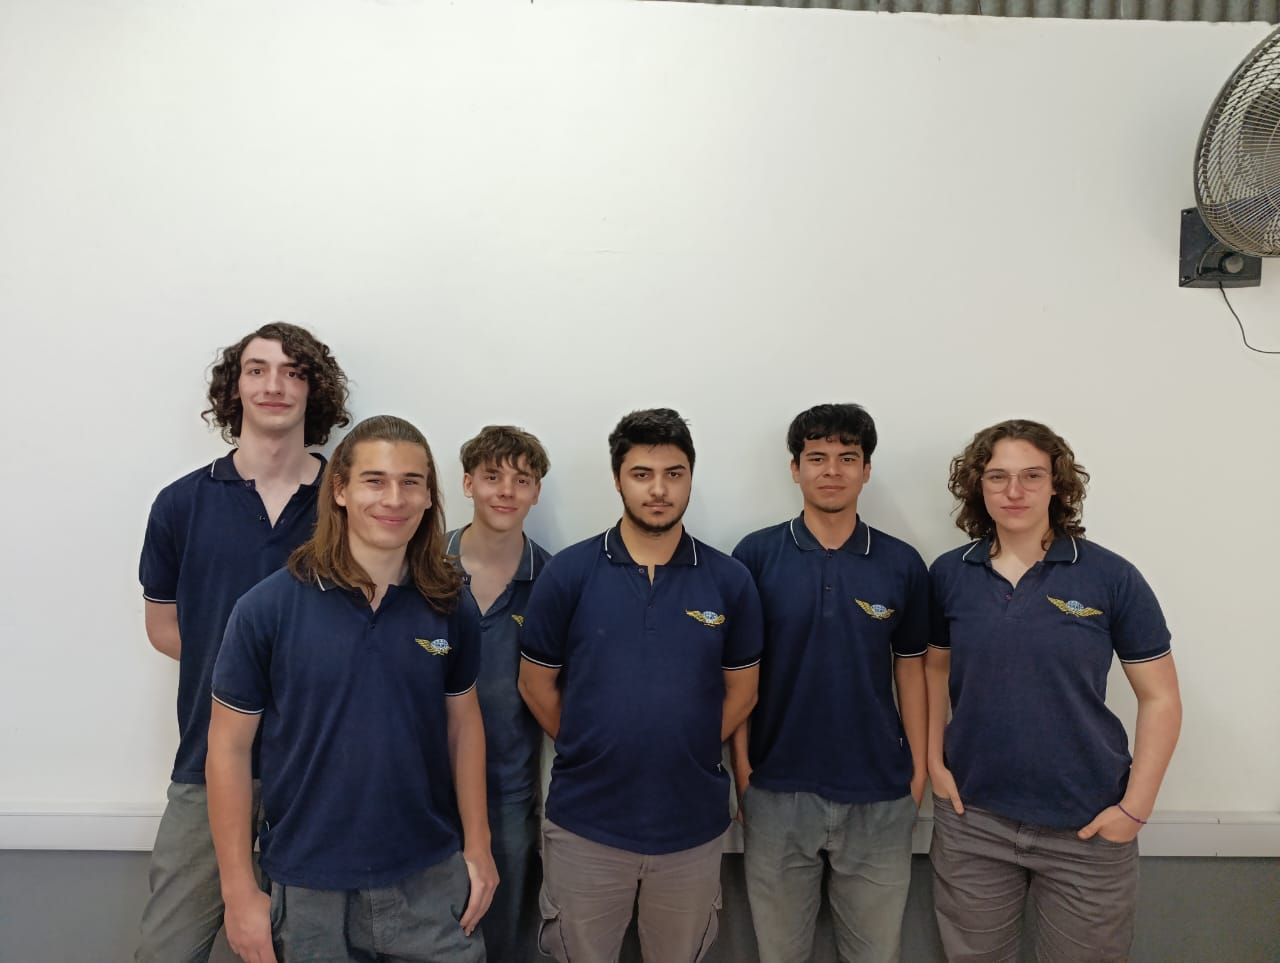
\includegraphics[width=\linewidth]{Preámbulo/Grupal.png}
                \caption{Grupo de \textcolor{dark_violet}{\textbf{GraviCap}}}
            \end{figure}
            \clearpage
        \section{Contacto}
            Mail de Contacto: \textcolor{light_violet}{\textbf{gravicap.arg@gmail.com}}\par
            Cuenta de Instagram: \href{https://www.instagram.com/gravi.cap/}{ \textbf{@gravi.cap}}\par
            Página Web: \href{https://gravicap.vercel.app/home}{\textbf{https://gravicap.vercel.app/home}}\par
            Repositorio de GitHub: \href{https://github.com/impatrq/gravicap}{ \textbf{https://github.com/impatrq/gravicap}}\par
            
        \section{Docentes a cargo}
            \begin{itemize} [label=•]
                \setlength{\itemindent}{1.5em}
                    \item Diego Palmieri
                    \item Carlos Bianco
                    \item Sergio Medina
                    \item Fabrizio Carlassara
                    \item Gabriel Argüello
            \end{itemize}
                
        \section{Agradecimientos}
            Agradecemos a la Asociación Cooperadora del \href{https://www.impatrq.com}{IMPA}.\par
            Agradecemos a \href{https://www.invap.com.ar}{INVAP} y al Ingeniero Marcelo Leo.\par
            Agradecemos a Impulsar por el panel solar.\par
            Agradecemos a todas los programas de difusión que nos brindaron el espacio para que podamos promover el proyecto.\par
            Agradecemos al personal docente y no docente de la institución por el apoyo inmenso que nos dieron.\par

        \section{Información Adicional}
            \subsection{Tiempo total de realización}
                \begin{itemize} [label=•]
                    \setlength{\itemindent}{2.5em}
                        \item \textbf{Día de Inicio}: 18/03/2024
                        \item \textbf{Total de Semanas para la finalización}: 30,28 semanas.
                        \item \textbf{Tiempo individual por semana}: 8 horas.
                        \item \textbf{Tiempo de realización en horas}: 243 horas.
                \end{itemize}
                
            \subsection{Lenguajes de programación utilizados}
                \begin{itemize} [label=•]
                    \setlength{\itemindent}{2.5em}
                        \item \LaTeX
                        \item C++
                        \item C
                        \item HTLM
                        \item CSS
                        \item Vue.js
                        \item React
                        \item Java
                        \item JavaScript
                \end{itemize}
                
                \subsection{Programas utilizados}
                    \begin{itemize} [label=•]
                        \setlength{\itemindent}{2.5em}
                            \item Overleaf
                            \item Visual Studio Code
                            \item Canva
                            \item MarvelApp
                            \item Photoshop
                            \item KiCad
                            \item Inkscape
                            \item Ionic
                            \item Putty
                            \item PlatformIO
                    \end{itemize}